\documentclass[conference]{IEEEtran}
\usepackage{graphicx}
\IEEEoverridecommandlockouts
% The preceding line is only needed to identify funding in the first footnote. If that is unneeded, please comment it out.
\usepackage{cite}
\usepackage{amsmath,amssymb,amsfonts}
\usepackage{algorithmic}
\usepackage{graphicx}
\usepackage{textcomp}
\usepackage{xcolor}
\def\BibTeX{{\rm B\kern-.05em{\sc i\kern-.025em b}\kern-.08em
    T\kern-.1667em\lower.7ex\hbox{E}\kern-.125emX}}
\renewcommand{\thesubsection}{\thesection.\alph{subsection}}
\begin{document}

\title{BareTag Tool-Tracker\\
{\footnotesize {Team 3 - University of Massachusetts Amherst Senior Design Project 2025 }}
}

\author{\IEEEauthorblockN{Walter Tebbetts}
\textit{CompE}\\
\textit{Software Lead}

\and
\IEEEauthorblockN{Sean Brown}
\textit{CompE}\\
\textit{Logistics Lead}

\and
\IEEEauthorblockN{Ken Su}
\textit{CompE}\\
\textit{Budget Lead} 

\and
\IEEEauthorblockN{Connor McGarry}
\textit{CompE}\\
\textit{Hardware Lead}

\and 
\IEEEauthorblockN{Jeremy Gummeson}
\textit{Professor, ECE}\\
\textit{Advisor}

}

\maketitle

\begin{abstract}
    Over the past 10 years, the majority of tools on a construction 
    site have converted from wired to battery-powered. While this 
    makes tools easy to move around, it also makes them easy to misplace
    and an easier target for theives. Data indicates that the construction
    idustry suffered nearly \$1,000,000,000 in loses due to tool theft in
    2016 alone [1], strongly indicating the need for a robust and effective 
    theft mitigation system. We propose the BareTag Tool Tracker, a novel
    approach to tool tracking that utilizes Ultra-Wideband(UWB) and Bluetooth 
    Low-Energy(BLE) radio in order to real-time track tools, materials, or other 
    valuable items on a construction site. The system utilizes a series
    of pre-placed Anchor posts, that send UWB pings to a Tag that is connected
    to a tool. Each Anchor can then calculate its distance to a Tag, relaying
    that information to a Base station over Long Range(LoRa) radio. The 
    base station runs the aggregated distance data through a multilateration
    algorithm that can calculate the Tag's location with 50 cm accuracy.
    The calculated location is then output to a local terminal, as well as 
    uploaded to a cloud database for future reference. Altogether, the BareTag Tool-Tracker
    is highly accurate (50 cm), low-power (1 year of battery life), and
    scalable (increase range by adding additional Anchors).
\end{abstract}


\section{Introduction}
Modern construction sites heavily rely on the usage of battery operated 
power tools, allowing construction workers to dynamically move throughout 
a site without the need to route cables and power lines for their 
equipment. This allows individual workers, as well as entire 
construction firms, to be more efficient, eliminating the need to set 
up power infrastructure at every new site, or re-work power infrastructure 
when a site changes. However, this flexibility and ease of use create new 
challenges to construction site efficiency. First of all, battery-powered 
tools are often smaller and easier to misplace compared to their corded 
predecessors, greatly reducing a firm’s overall efficiency. Second, 
battery-powered tools are very valuable, with many cordless power tools 
costing \$800+, greatly increasing the incentive for thieves to steal 
cordless tools and accessories. In order to prevent inefficiencies caused 
by misplaced tools and to deter common tool theft, a precise and scalable 
tracking system needs to be implemented for the construction industry. 
With this project, we propose a system that combines functionality of 
existing item tracking and inventory management solutions, into a highly 
precise and scalable solution specifically tailored to the construction 
industry. While this solution is focused on preventing tool misplacement 
and theft, we have also designed the system to be flexible, allowing 
users to utilize the system to track and monitor equipment, materials, 
or even individuals.

\subsection{Significance}

In 2016 it was estimated that in the United States alone \$1,000,000,000 
worth of construction tools were stolen [1]. A survey by the Charted 
Institute of Building discovered that out of the 1000 construction mangers 
interviewed, a third responded that they had experienced theft weekly on 
their sites. It was estimated that each of these weekly incidents cost the 
business an average of \$6,000, in some cases, in a single night the site 
had lost \$100,000 worth of equipment [2]. What’s worse is that this is a 
growing case. The FBI has reported that in 2021, theft on construction 
sites had outgrown theft in convenience stores [3]. Many managers have 
reported that these incidents have escalated to organized crime with 
evidence of sophisticated planning and coordinated executions. [2]. 
Theft on the site is not only costly to the business owners but also 
inconvenient for the construction workers and their managers. 
Due to the lack of proper tools construction workers may not continue with
their assignments and managers have to keep pushing deadlines. The 
result of this costs the business not just in extra wages, but also 
extra insurance and reputation [2]. 

\subsection{Context and Survey of Similar Solutions}

The general problem of item tracking has had many attempted solutions 
and continues to be a problem of interest today. In designing our system, 
we extensively researched many similar solutions to examine how these 
solutions fall short of achieving our system’s goals. Other solutions 
we have examined use various technology for tracking such as: AI image 
processing, GPS, Bluetooth, and Ultra-Wideband.

One comparable solution that utilizes image processing methods is offered 
by SIRIX. Their approach involves human and AI-assisted item tracking, 
using two types of cameras: wide-angle and thermal. These cameras are 
strategically placed throughout the job site and are monitored 24/7 by both
human operators and AI [4]. However, this solution is highly unreliable 
and unsustainable due to the presence of blind spots that fall outside 
the cameras' field of view, leaving certain areas unprotected. 
Additionally, human judgments and AI decision-making can introduce 
further response time, potentially allowing thieves to escape with 
stolen items before any alert is triggered. Another concerning issue 
is with the way that the system is powered. Attackers, especially a 
criminal organization as mentioned in the problem statement could easily 
disable the system by cutting the power generator or energy source, 
rendering it inoperative, leaving the remote surveillance team with no 
recourse other than calling the authorities. While both SIRIX and 
BareTag offer 24/7 security systems, only BareTag qualifies as a 
true round-the-clock security measure. BareTag does not depend on 
human or AI intervention to ensure tools and materials are secure. 
Additionally, BareTag's low power consumption allows it to operate 
more efficiently across diverse terrains, offering higher portability 
and flexibility compared to the energy-intensive SIRIX system.

Another comparable solution we evaluated is a commercial system called 
GoCodes, which specifically addresses the issue of tool tracking. This 
system employs continuous GPS tracking to monitor valuable equipment 
within a geofence, helping businesses prevent the loss or theft of tools. 
While it offers effective on-site tracking, off-site tracking relies on 
individuals scanning QR codes placed on the tools. If a user scans the 
QR code, the item's location outside of the geofence can be updated [5]. 
However, this approach has a significant flaw — no tool thief would 
voluntarily scan the QR code, and they could easily remove the codes 
from the tools, eliminating any trace of the theft. Although GoCodes 
provides a workable solution, it has several drawbacks that our system 
aims to overcome. For one, GPS tracking is power-intensive, often requiring
frequent battery replacements for the trackers. Additionally, GPS 
tracking needs an unobstructed line-of-sight to function efficiently, 
which can be compromised in dynamic construction environments. 

Another popular solution is the Apple AirTag.
The Apple AirTag, uses Bluetooth Low Energy (BLE) advertisements to connect
with devices in the Find My network (iPhone, iPads, and Macbooks). 
Additionally, it uses UWB to allow users to get a more accurate location of where 
the Tag is once the AirTag is close enough to the owner's iPhone [6]. This 
creates a well-rounded system to let users get a general idea of where 
their items are with a battery life of up to one year. The difference 
between the BareTag and the AirTag is that the BareTag is used for 
accurately tracking high-value items within the set UWB perimeter. 
BareTag emphasizes the use of the UWB module so construction workers 
can easily find their tools, along with an additional BLE module for 
the Find My network features outside of the set perimeter. Unlike AirTag, 
our system aims to not only track and retrieve items but also to accurately 
and reliability track tools to optimize efficiency.

The final solution, Pozyx, is most similar to the BareTag. Pozyx tracks 
items indoors by installing UWB Anchors throughout the building, which 
communicate with UWB Tags. These Anchors are height-adjustable and 
plugged into walls. Once configured and registered in the system, 
items can be geofenced, and the collected data can be used to optimize 
workflow and labor efficiency [7]. While Pozyx offers an effective 
indoor tracking solution, it is less efficient in outdoor environments. 
In locations like construction sites, where power availability may be 
limited, Anchor placement becomes a significant challenge. In contrast, 
BareTag’s Anchors are battery powered and easy to reconfigure, 
making the system more portable and scalable. 
Furthermore, BareTag’s Tags feature a built-in accelerometer with an 
automatic sleep function to maximize power efficiency. This not only 
extends battery life but also reduces the frequency of battery 
replacements, saving time and resources. In summary, BareTag's Anchors 
do not rely on external power sources, and the Tags are equipped with a 
low-power solution, making them more suitable for outdoor construction 
site use compared to Pozyx.

\subsection{Societal Impacts}

Our system can positively benefit all of society. As a tool tracking 
system made for construction workers, they are the most obvious group 
of people who benefit from this system. With construction workers being 
the primary users of our system, many of our design choices will be made 
specifically for the system to be easily used by the average construction 
worker. We want to create a user-interface that helps construction workers 
track their tools without having to do any additional work of their own. 
While this will greatly help construction workers find their tools and 
not have to worry about their tools being stolen, it benefits owners of 
construction firms even more. With accurate tool tracking, they can 
ensure their workers are working as efficiently as possible and not 
wasting their time looking around sites for tools. Owners of construction 
companies are also the ones responsible for supplying their workers with 
the tools needed to complete jobs. We want our system to reduce these 
costs for construction firm owners by reducing the loss and theft of 
their very expensive tools. Preventing theft and increasing the 
efficiency of workers can help a construction firm look more professional 
and hireable by employers that need construction work done. Our system 
aims to help construction teams work quicker to efficiently finish jobs 
which will increase the number of jobs they can take. Because our system 
increases construction efficiency, anyone benefiting from the construction 
of literally anything can benefit from it as well. The only people that 
will be hurt by our system are thieves that will be caught stealing 
expensive tools by our system.

\subsection{Goals, Specifications and Testing Plan}

The BareTag Tool Tracker will implement the following goals, 1. Real-time 
tracking within a specified zone, 2. Precise accuracy for tracking within 
the zone, 3. Low Power,  4. Reliability outside the zone, 5. Scalability.

The specifications listed in Table 1 demonstrate the goals that our project 
aims to achieve by the time that we have a finalized product.
\begin{center}
\begin{table}
\caption{Design Goals and Testing Plan}
\begin{tabular}{|p{4cm}|p{4cm}|}
    \hline
    \textbf{Specification}  & \textbf{Testing Plan}\\
    \hline
    The system will track an item’s geo-coordinates with a reliability of 
    95\% within a specified 100 m x 100 m zone. 
    &
    Ping the Tag at randomized coordinates within the Sustainable 
    Engineering construction site.\\
    \hline
    The system will have less than 50 cm precision for tracking within 
    the specified zone.
    &
    Compare Tag’s measured location to its actual location 
    within a predefined grid.\\
    \hline
    The system will operate 24/7 for ~1 year without 
    replacing the batteries.
    &
    Measure the power consumption of the system in multiple modes.\\
    \hline
    Ensure that the Tag can be tracked via the Find My network outside 
    of the UWB zone.
    &
    Confirm tracking accuracy in scenarios with different saturations 
    of Find My devices by comparing with AirTags in the same location.\\
    \hline
    Able to increase range of the UWB perimeter by adding more Anchors.
    &
    Demonstrate that a Tag’s trackable range in the UWB zone increases 
    when adding a new Anchor.\\
    \hline
    Create a user-friendly GUI that displays geographical locations of multiple Tags.
    &
    Have a non-team member use our application and easily track Tags spread around a zone.\\
    \hline
\end{tabular}
\end{table}
\end{center}


\section{DESIGN}

This section describes the system design including design alternatives, 
design justifications, and hardware and software block diagrams.

\subsection{Overview}
At a high level, the BareTag Tool Tracker utilizes Ultra-Wideband (UWB) and 
Bluetooth Low Energy (BLE) radio in order to real-time track an 
item's location on a construction site. The technology at the core of our 
design is UWB radio. UWB radio is a form of radio communication that 
utilizes pulses of radio energy at specifically timed intervals in order 
to transmit information. This protocol is not ideal for data communication, 
but is very accurate in performing distance ranging. With two UWB 
transceivers, one configured as the controller (Anchor) and the other 
configured as the responder (Tag), the Anchor can range it's distance
to the Tag via UWB pings. The Anchor begins by sending a ping with 
the desired Tag's ID encoded, the Tag will almost immediately send 
back a response ping, the Anchor can then use the time between when it 
sent its ping to when it received the Tag's ping, in order to 
calculate the distance between the two transceivers. 

\[ d = \frac{\frac{ToF}{2}}{c} \]

Where $d$ is distance between the Anchor and Tag, 
$ToF$ is time of flight, and $c$ is the speed of light.

With distance measurements between 3 Anchors and 1 Tag, we
can preform a trilateration algorithm in order to calculate
the Tag's location within our site.

The equations for the three circles (Anchor to Tag distance):

\[(x - x_1)^2 + (y - y_1)^2 = r_1^2\]
\[(x - x_2)^2 + (y - y_2)^2 = r_2^2\]
\[(x - x_3)^2 + (y - y_3)^2 = r_3^2\]

Where $r_i$ is the distance from an Anchor to a Tag, $(x_i, y_i)$ are 
the cordinates for each Anchor on a 2D $x,y$ plane, and $(x,y)$ are the coordinates
for the Tag we are trying to locate.\\
Next we subtract the second equation from the first:

\[(-2x_1 + 2x_2)x + (-2y_1 + 2y_2)y = r_1^2 - r_2^2 - x_1^2 + x_2^2 - y_1^2 + y_2^2\]

Likewise, subtract the third equation from the second:
\[(-2x_2 + 2x_3)x + (-2y_2 + 2y_3)y = r_2^2 - r_3^2 - x_2^2 + x_3^2 - y_2^2 + y_3^2\]

Re-writing these two equations using A, B, C, D, E, and F:
\[Ax + By = C\]
\[Dx + Ey = F\]

Finally, the Tag's $(x,y)$ coordinates are:
\[x = \frac{CE - FB}{EA - BD}\]
\[y = \frac{CD - AF}{BD - AE}\]

Once the Tag's location has been calculated via our trilateration algorithm,
the Tag's location will be output to a local terminal, as well as 
uploaded to a cloud database. Outputting to a local terminal allows us to
have the system function without the need for an internet connection, 
something that may not be available on rural construction sites. If internet
is available, we can upload location to cloud database. With location data
stored remotely, any user with internet access can get their Tag's current
location, or past location.

Aditionally, as one of our main goals is to prevent theft, when a Tag
leaves the designated construction site, a notification will be sent to 
the user, letting them know that one of their Tag's has left the site.
To continue to track the Tag once it leaves the construction site, we will
turn off the Tag's UWB radio, and turn on the Tag's BLE radio. Using BLE
advertisements, the Tag will be able to communicate with nearby devices that
are using the Apple Find My protocol. The Find My protocol allows BLE devices
to be tracked with around 10 meter accuracy when in loactions saturated with 
Apple devices. With this tracking outside of the construction site, users 
can not only keep track of their tools on a construction site, but also track
down stolen tools outside of the construction site. To help integrate our
Tags into the Find My network, we will be using the open source project,
openhaystack. 

Openhaystack, is an open source project originating from TU Darmstadt, that
utilizes Find My's open API, as well as a collection of reverse engineering
and security analysis work to allow generic BLE devices to be tracked via
Apple's Find My network.

Altogether, the BareTag Tool Tracker utilizes UWB and BLE in order to real
time track the location of Tags on and off a construction site. The design
combines existing solutions for item tracking with UWB as well as the robust
and expansive Find My network to prevent tool theft and increase construction
site efficiency.  

\begin{figure}
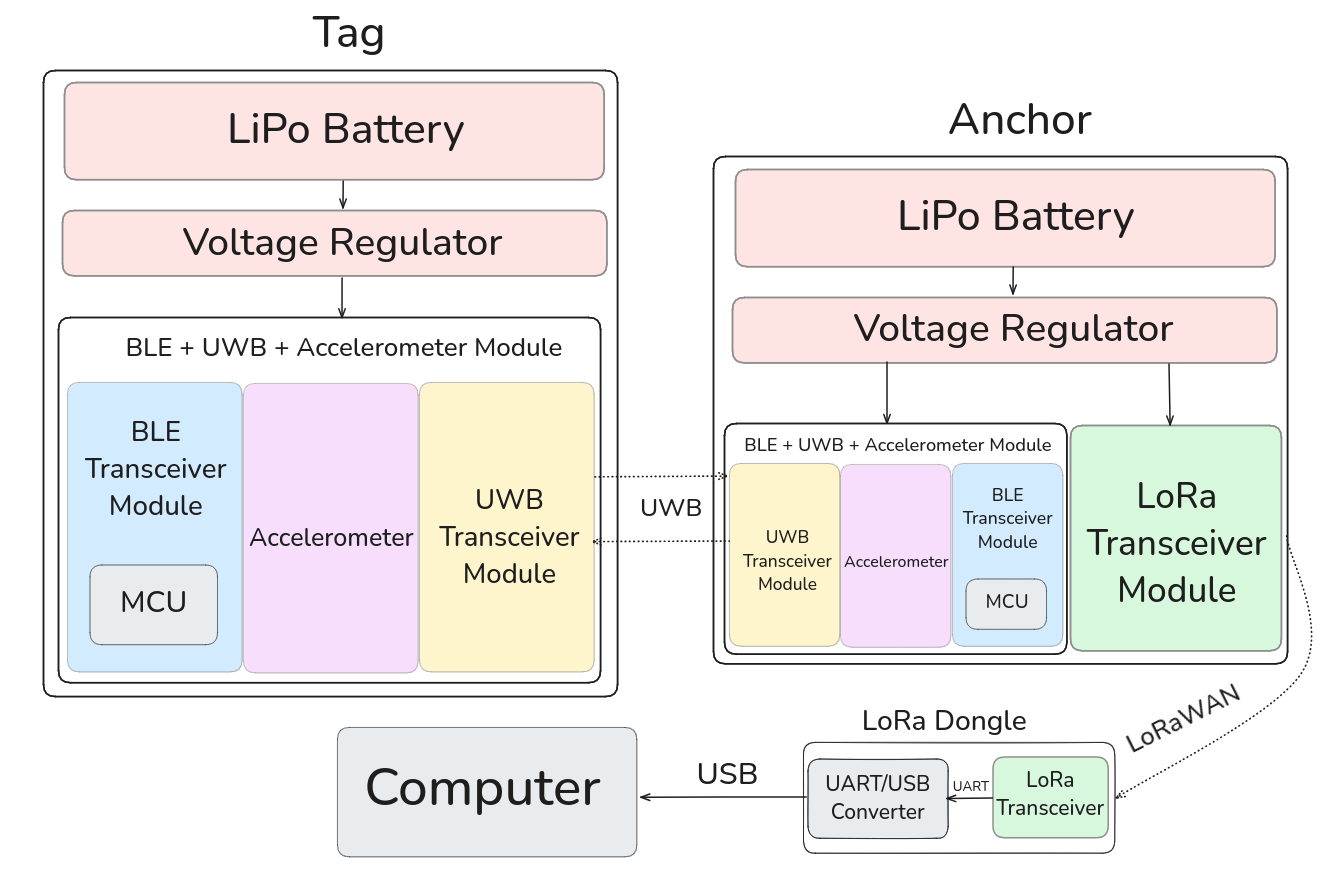
\includegraphics[scale=0.185]{Screenshot from 2024-10-18 21-37-02.png}
\caption{Full system hardware block diagram}
\end{figure}

\subsection{Tag}\label{AA}
The Tag refers to the trackable device that will be attached to the tools 
on a worksite. The goal is for the Tags to be less than $31.9mm^2$, which is 
of a similar size to the Apple AirTag. The thickness of the Tags is aimed 
to be under $16mm$, with the primary contributor to this size being the 
pouch cell $290mAh$ Lithium Polymer battery. The peak current draw of the 
Tag is $45mA$ and is out of the range that a coin cell could support, 
which led to the decision to use a LiPo that fits within our area size 
goals at $25 \ mm \ x \ 28\ mm$. We are aiming for a one year battery life.
\\The primary part of the Tag is the Qorvo DWM3001C. This module is driven 
by the nRF52833 MCU which includes BLE functioality. The DWM3001C also includes, 
UWB and accelerometer modules. The UWB functionality is driven by the DWM3110,
which has an integrated PCB antenna. BLE is provided by the nRF52833. This MCU is built on an ARM Cortex 
M4 and operates at $2.4GHz$. This MCU is programmable over 
SWD and thus requires a corresponding interface to be added to the PCBs. 
The accelerometer is the LIS12DH, and is used to wake up the module 
upon motion detection. The module will set the interrupt pin on the 
DWM3001C high when there is motion detected. Otherwise, the Tag is in a 
low power mode and is not receiving UWB pings. 
Therefore, before the Tag goes to sleep the location needs to be checked 
to determine the last known resting location. The Tag has the BLE radio turned off 
until it exits the UWB area, at which point an interrupt pin turns 
it on to integrate the Tag into the Apple Find My network. At this point, the 
UWB module turns off to conserve power. The accelerometer still regulates 
the power mode of the Tag depending on motion to conserve power. This
device draws a lot of concepts from ECE 523 and ECE 304, both of which 
have a heavy focus on minimizing power consumption via software and 
component selection. The TPS79933 voltage regulator has an output of 
$3.3V$ when the input voltage is over $3.475V$. This component is used in 
both the Tags and Anchors as both devices operate on a $3.7V$ battery 
with all modules operating at a $3.3V$ ideal voltage. 


\subsection{Anchor}
There needs to exist at least $3$ Anchors for the coordinates of a Tag to be 
transmitted to the Host Device, which are calculated through multilateration. 
The Anchors use the same Qorvo DWM3001C modules as on the Tags as all 
of the submodules have a use case here too. The Anchors use UWB to ping 
the Tag and determine its location within the area defined by the 
proximity of the other Anchors. They process this data using the 
nRF52833 MCU and send it to a host device over LoRaWAN for coordinate computation. 
The RYLR998 LoRa module in the Anchors operates within the operating range of 
LoRaWAN: $902.3 MHz$ to $914.9 MHz$. This module communicates with the MCU 
via UART. The use of these LoRa modules means that the Host Device does 
not need to be on the site of the construction due to the 
kilometers of range that LoRa supports. We will build the LoRaWAN 
protocol on top of LoRa using the nRF52833 MCUs and Host Device. The use of the nRF52833 
means that we can take advanTage of the BLE it provides and use 
it for a variety of functions. The GPS coordinates of the Anchors must 
be known in order to get the real-world position of the Tags, and we can achieve
this through a mobile app that will communicate with the Anchors over Bluetooth. 
This operation will occur during the setup and positioning of the Anchors. We can also
use BLE to communicate with an Anchor to alert that a Tag in 
BLE mode has been returned within range of the Anchors. These features 
result in  more power consumption than the Tags, so a 2.2Ah Lithium Ion 
battery is used. This is possible due to less size constraints for the 
Anchors than of the Tag. The Anchors are not constrained by size, and therefore we 
do not have any strict specifications for its dimensions.
As stated before, the TPS79933 voltage regulator outputs 3.3V, which is 
the ideal operating voltage for the DWM3001C and LoRa module. 


\subsection{Lora Dongle}
This device is a RYLR998 operating over a USB/UART connection with the 
Host Device. The Dongle allows the Host Device to receive the Tag location data in 
reference to each Anchor, which the Host Device will then perform the multilateration algorithm on.
The size of this device should be similar 
to that of a commonly used USB hub, as to not be an inconvenience to have attached to a 
small host device. The dimensions will be approximately $32 \ mm\  x \ 18 \ mm \
x \ 8 \ mm$ based on a combination of the Dongle component dimensions, which are the LoRa 
module and a USB/Serial converter. 
\\ The Dongle receives power over USB from the Host Device, which the serial converter will
drop to $3.3V$ for the ideal operating voltage of the LoRa module.

\subsection{Host Device}

This device can be whatever system a supervisor desires to use as long as 
it can support a USB/Serial connection, or do so using adapters. The Host Device
performs the multilateration algorithms based on the data it receives from the LoRa Dongle.
The calculations get backhauled to a cloud database 
where the history of Tag locations can be mapped out to determine 
daily paths. This information is also displayed locally on a map of 
the desired area. The Host Device is also running the macless-haystack 
server, which acts as a means for tracking the Tags that have 
left the UWB area and are using BLE to integrate with the Apple Find 
My network. The Tags all have unique IDs that can be linked to tools or 
equipment, making it easy to parse the data and determine what items have 
been in what location. 
\subsection{3D Localization}
To find the z-coordinate of the Tag using only three Anchors, 
we need the distances between the Anchors and the distances between 
the Tag and Anchors. The shape the Anchors and Tag form is known as a 
tetrahedral. Using the volume and the base area of the tetrahedral we 
are able to find the height which represents the Tag’s z-coordinate. 
In [8] we know that using Heron’s formula on the distances between the 
Anchors we can get the area of the base
\[S_{ABC} = \sqrt{(p - AB)\cdot(p-AC)\cdot(p-BC)}\]
and using Euler’s formula we can get the volume of the tetrahedral.
\[V_{HABC}^2 = \frac{1}{36}
\begin{vmatrix}
    a^2 & \frac{a^2+b^2-n^2}{2} & \frac{a^2+c^2-m^2}{2} \\
    \frac{a^2+b^2-n^2}{2} & b^2 & \frac{b^2+c^2-l^2}{2} \\
    \frac{a^2+c^2-m^2}{2} & \frac{b^2+c^2-l^2}{2} & c^2
\end{vmatrix}\]

By rearranging the formula for finding the volume of a pyramid
\[V_{HABC} = \frac{1}{3}S_{ABC} \cdot H\]

we get the height of the tetrahedral as a function of volume and base.
\[H = 3 \cdot \frac{V_{HABC}}{S_{ABC}}\]
Then, using the volume and area that we previously calculated, 
we get the height of the tetrahedral, which is also the z-coordinate of
the Tag. To validate that this method works we ran a simulation through 
Blender and confirmed that the equations do indeed give us the correct 
z-coordinate.

\section{THE PROTOTYPE}
\subsection{Prototype Overview}
The prototype currently consists of 3 hardware components, each with 
associated software to control their functionality. The 3 hardware 
components are the Tag, the Anchor, and a LoRa dongle connected to the 
host computer.
The Tag consists of a DWM3001C UWB, BLE, and IMU combo module, along with 
associated programming headers, debug LEDs, and a 290 mAh LiPo battery. 
The DWM3001C allows us to use one module as our MCU and host device for 
all radios and other peripherals required for our design. The DWM3001C 
along with associated passive components are mounted on a custom SMT PCB 
to make the Tag. 
The Anchor also consists of a DWM3001C, as well as a RYLR998 LoRa radio, 
along with a programming header, debug LEDs, and a 2200 mAh LiIon battery. 
The RYLR998 is a hobbyist LoRa radio that allows us to transmit 256 byte 
packets wirelessly from our Anchors to the host computer. These packets 
communicate measured distance between Anchor and Tag, as well as data about 
the current state of the Anchor. Same as the Tag, the DWM3001C and RYLR998 
along with associated passive components are housed on a custom SMT PCB to 
make the Anchor. Anchors are mounted on metal poles that allow for fast 
reconfiguration and ease of testing indoors and outdoors. 
The LoRa dongle connected to the host computer is a generic USB TTL to 
UART converter connected to a RYLR998. The host computer runs a custom 
Python script that gathers distance data from all 3 Anchors to perform a 
trilateration algorithm to pinpoint the Tag’s current location. Anchors 
run a custom firmware that has them send a UWB ping to the Tag around once 
every second. A randomized delay is put between pings in order to prevent 
two different Anchors from pinging the Tag at that same time. Once receiving 
a distance measurement from the Tag, each Anchor relays this information to 
the host computer using the RYLR998, controlling the module over UART. The 
Tags run a simple custom firmware, responding to UWB pings whenever one is 
received. Combining these hardware and software components we get a complete 
prototype that can find a Tag’s location in real time with 50 cm accuracy.

\subsection{List of Hardware and Software}
Hardware:
\begin{itemize}
    \item Qorvo DWM3001C
    \item Reyax RYLR998
    \item 3.7V 290mAh LiPo
    \item 3.7 2200mAh LiIon
    \item USB-A to UART Converter
    \item Raspberry Pi 4B
    \item Tag-Connect Edge-Connect Programmer
    \item SEGGER JLink Edu Mini
\end{itemize}

Software:
\begin{itemize}
    \item Docker
    \item Xcode
    \item Serial Monitor
    \item Debian Linux
\end{itemize}

\subsection{Custom Hardware}
We designed two custom PCBs to act as the Tag and Anchors of our system. 
In our current system, we were able to trilaterally locate the custom PCB 
Tag with 3 Anchors: two Qorvo DWM3001CDK development boards and one of our 
custom PCB Anchors. Our main goal when creating our Tag PCB was to make it 
as small as possible. We eventually want these Tags to be placeable inside 
of tools. In our first revision, we were able to minimize the size of the Tag 
to approximately 26.8 by 31.6 mm squared. We were also able to successfully 
program our DWM3001C with the Edge-Connect seen in Fig. 4 attached to the 
castellated edges of our Tag PCB. Because of this, we will be able to remove 
the 10-pin programming header seein in Fig. 2 to reduce the size of the Tag 
PCB in our second revision.

While the Tag and Anchor PCBs look quite different, they are populated with 
very similar components. The major difference between the two is the LoRa 
module that can be seen extending off the left side of the Anchor PCB in Fig. 
4. The LoRa module on the Anchor is used to communicate distance  measurements 
from the Anchors to a base station in order to perform our trilateration 
algorithm and locate the Tag.

While we were able to integrate our PCBs to make a functioning system, we 
still had some issues that we plan to address in our next revisions. The 
battery connectors into the PCBs on the Tags and the Anchors are facing 
into other components on the board, making it difficult to connect and 
disconnect our batteries to them. Our LEDs were meant to flash during 
transmission and reception of Ultra-Wideband pings on the Anchor and the 
Tag. While this was not achieved, the main functionality of our PCBs were 
not impacted. The UWB antenna on the Anchor PCB is on the opposite side of 
the LoRa antenna because we were originally worried about signals interfering 
with each other from the two different modules. In our next revision, we will 
have both antennas facing up to have them in their ideal orientation for 
transmitting and receiving signals. With this modification, we will be able to 
maximize the area where we can precisely locate our Tag with Ultra-Wideband 
pings. As you can see in Fig. 2 and Fig. 3, there are many more components on 
each of our boards. These include resistors to limit current flow into certain 
components, capacitors to reduce noise from input voltage, and LEDs that were 
meant to be used to help us debug our system. Most importantly, we had a 
voltage regulator to limit the input voltage into our Qorvo module to its 
preferred 3.3 volts. We also have many test points that helped us debug our 
system which we will remove in future revisions. Overall, our first revisions 
of our custom PCBs worked well enough for our prototype to function properly.

\begin{figure}
\begin{center}
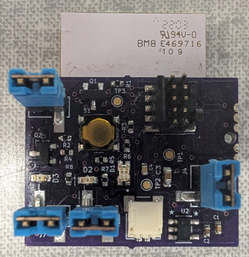
\includegraphics[scale=3]{mdr_tag_picture.png}
\caption{Populated Tag PCB}
\end{center}
\end{figure}

\begin{figure}
\begin{center}
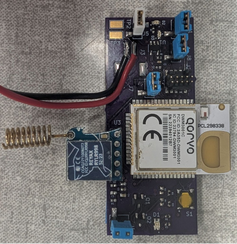
\includegraphics[scale=3]{mdr_anchor_picture.png}
\caption{Populated Anchor PCB}
\end{center}
\end{figure}

\subsection{Prototype Functionality}
In accordance with our hardware block diagrams in Fig 2, the PCBs all work 
as intended. The modules and batteries communicate as per design. Fig. 4 
depicts the Edge-Connect programmer pins pressed to the edge of the Tag PCB. 
This method of programming proved to work, and we were successfully able to 
flash firmware to the nRF52833.

\begin{figure}
\begin{center}
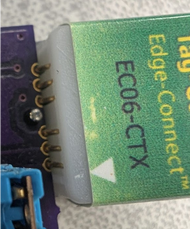
\includegraphics[scale=1]{mdr_edge_connect.png}
\caption{Edge-Connect Programmer on Tag castellated edges}
\end{center}
\end{figure}

\subsection{Prototype Performance}
Our Prototype met all of our proposed MDR deliverables. We were able to 
integrate our two custom PCBs into our proposed system to track one custom 
Tag. Although the LEDs on our PCBs did not function properly, they did not 
cause any performance issues. Looking back at our complete design 
specifications, our current Prototype is well on its way to achieve them. 
For starters, we were able to track a Tag with 50 cm accuracy within a 
predefined 10 x 10 m zone. Although this is much smaller than our system’s 
final goal, we believe that we could have had a larger range if we had the 
space to do so. Our system was also capable of tracking a Tag outside the 
UWB zone using the Apple Find My network. A major performance metric that 
we evaluated is the battery life of our system. As previously stated, our 
design goal is to have an available system for ~1 year without the need for 
replacing any batteries. To test our current system’s battery life, we 
analyzed the current draw of our devices when the system was operating. 
Fig. 5 shows the power consumption of our singular Tag PCB while it is 
only transmitting Bluetooth Low Energy signals. For the majority of the 
time, the Tag is idle, but it wakes up and sends a bluetooth signal 
approximately every 5 seconds. In BLE mode, our Tag consumed 60.73 
microamps, giving it an approximate battery life of 200 days with a 
290 mAh battery attached to it. This was the expected power consumption 
for our Tag in BLE mode. While our Prototype’s battery life performed well 
in BLE mode, it did not perform close to how we want it to when sending 
Ultra-Wideband pings. In Fig. 6, the power consumption of the Tag in UWB 
mode can be seen changing as it switches from waiting to receive UWB pings 
to sending them. Our Tag in UWB mode has an average current draw of 51.63 
mA. With the 290 mAh battery our current system has attached to a Tag, its 
battery life is under 6 hours. This battery life is well below our system’s 
desired battery life, but there are many software power optimizations possible
for our system.

\begin{figure}
\begin{center}
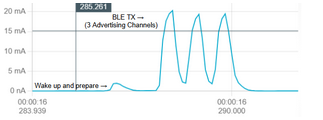
\includegraphics[scale=1]{mdr_ble_power_consumption.png}
\caption{Power consumption of Tag in BLE mode}
\end{center}
\end{figure}

Lastly, we analyzed the power consumption of one of our Anchors. 
Similarly to the Tag, our custom PCB Anchor had an average current 
consumption of 49.23 mA. The Anchor acts as the main transmitter of the 
signals while the Tag is the main receiver. Although our Anchor has a 
similar current draw, it has a much longer battery life because our 
current Anchor has a 2200 mAh battery attached to it. We are less worried 
with the current draw of our Anchors because they are not size constrained, 
allowing us to connect many batteries to them. 


\begin{figure}
\begin{center}
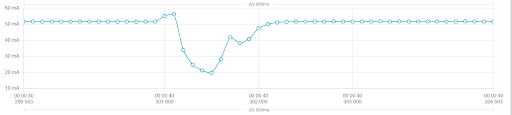
\includegraphics[scale=0.45]{mdr_uwb_tag_power_consumption.png}
\caption{Power consumption of Tag in UWB Mode}
\end{center}
\end{figure}

\begin{figure}
\begin{center}
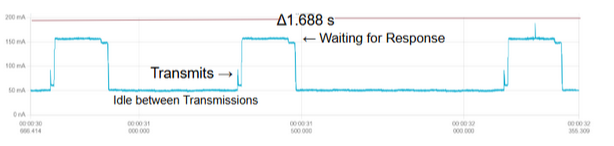
\includegraphics[scale=0.45]{mdr_uwb_anchor_power_consumption.png}
\caption{Power consumption of Anchor in UWB Mode}
\end{center}
\end{figure}

\section{CONCLUSION}
As of now, the project operates in the following states:
\begin{itemize}
    \item Full programming control over Tag and Anchor rev.1 PCBs
    \item Tag lasts 4775.23 hours in BLE mode
    \item Tag lasts 5.62 hours in UWB mode
    \item Anchor lasts 44.7 hours
    \item Anchors send Tag location over LoRa to host device
    \item Find My server runs on Raspberry Pi
\end{itemize}

\section*{ACKNOWLEDGMENTS}
We thank our advisor Professor Jeremy Gummesson for the endless 
advice and support throughout the design process. We also thank 
our evaluators Professor Tilman Wolf and Professor David McLaughlin 
for essential feedback from each quarterly presentation. Of course, 
thank you to all of the course coordinators for ensuring that the 
necessary support has been available. Additionally, thank you to 
Baird Soules and M5 staff for supplying a productive engineering 
environment for prototyping and rework, and for many important 
components that we used in our project.


\begin{thebibliography}{00}
\bibitem{b1} ``2016 equipment theft report,'' 2016. [Online]. Available: https://www.ner.net/wp-content/uploads/2017/10/Annual-Theft-Report-2016.pdf. Accessed Oct. 19, 2024.
\bibitem{b2} ``Crime in the construction industry,'' 2013. [Online]. Available: https://www.ciob.org/sites/default/files/. Accessed Oct. 19, 2024.
\bibitem{b3} ``An exploratory look at thefts from construction sites,'' 2019. [Online]. http://ascpro0.ascweb.org/archives/cd/2019/paper/CPRT247002019.pdf. Accessed Oct. 19, 2024.
\bibitem{b4} ``Remote Video Monitoring,'' SirixMonitoring, Sep. 13, 2024. [Online]. Available: https://sirixmonitoring.com/remote-video-monitoring/. Accessed Oct. 04, 2024.
\bibitem{b5} ``Pros and Cons of Construction Equipment Tracking,'' Tool Tracking Software, Aug. 02, 2023. [Online]. Available:  https://gocodes.com/equipment-tracking-pros-cons/. Accessed: Oct. 04, 2024.
\bibitem{b6} ``AirTag VS GPS tracker, what is the difference ?,'' Beepings.com, 2021. [Online]. Available:https://beepings.com/airTag-vs-tracker/. Accessed: Oct. 04, 2024.
\bibitem{b7} ``Pozyx UWB Tags - Accurate ultra-wideband trackers,'' Pozyx.io, 2024. [Online]. Available: https://www.pozyx.io/products/hardware/. Accessed: Oct. 04. 2024.
\end{thebibliography}
\vspace{12pt}

\section*{Appendix}
\setcounter{subsection}{0}
\subsection{Design Alternatives}
Before settling on our current design, we considered many alternatives. 
In order to make our user-interface have real world terrain displayed 
while tracking our Tags, we need to find the coordinate positions of our 
Anchors. In order to do this, we originally considered putting GPS 
modules on our Anchors, but decided instead on creating a mobile app 
that can be used to find the GPS of your phone when setting up the 
Anchors. We decided on this in order to save money, as individual GPS 
modules range from \$20-\$40. We also considered purchasing a separate 
MCU, LoRa, and UWB module to design our Anchor PCBs. We found this 
design too complex and instead decided on the same module as we are 
using in the Tags. We decided on this current design because we want 
the Tags and Anchors to have the same technology to be able to program 
them with the same libraries in order expedite software development. 
Batteries have been a prominent part of our design that we have put a 
lot of effort into deciding on. Because we want the Tags to be small 
enough to go inside of tools without manufacturers having to add room 
for them, we decided on very small batteries inside the Tag. We also 
considered doing energy harvesting for the Anchors to increase the 
battery life of them, but have decided on large batteries for the 
Anchors because they are less size constrained compared to the Tags. 
In our original plan, we were going to backhaul our data to a 
self-hosted database in order for processing. After some consideration, 
we decided that sending the data to a cloud database, such as AWS, 
would be more beneficial for our project. Using a cloud server will 
allow for scalability, decrease in cost, higher reliability, and 
greater performance than a database we could host in-house. The cloud 
database will also be easier for us to use because it comes with 
pre-existing features that will make project integration easier.

\subsection{Technical Standards}
Bluetooth Low Energy, specified by IEEE 802.15.1, is used for our Tags to 
communicate with nearby Apple Find My ‘finder’ devices to send data to the 
Apple Find My network for global location tracking.

Ultra-Wideband is used by our Tags and Anchors for local location tracking 
with 50cm accuracy. Our application of UWB is specified in IEEE P802.15.14, 
which describes UWB used for Ad Hoc precision tracking. This spec builds on 
other specs of importance such as IEEE 802.15.4.

LoRa, discussed in IEEE spec P1451.5.5 , is used for sending data to the 
Base Device. We have chosen to not implement LoRaWAN due to the features of 
our transceiver modules, the minimal amount data we are sending, and a desire 
to not use additional hardware such as a LoRaWAN gateway.

Our chosen RF emitters all adhere to FCC guidelines as defined in FCC 47 
CFR Part 15, which states that any radiator must be licensed unless it
meets 47 CFR 15, unless otherwise given specific approval by the FCC. 
FCC certifications can be found on the product pages for all of our 
hardware radiators.

\subsection{Testing Methods}
Apple Find My integration has been tested through validating location 
data displayed on a locally hosted GUI provided by [9]. 

UWB tracking has been tested with 3 Anchors and 1 Tag as of MDR. 50cm 
accuracy has been noted. This was performed through the manual creation 
of a coordinate system in an indoor open-field environment, and moving 
the Tag to different positions in the grid.

\subsection{Project Expenditures}
\begin{center}
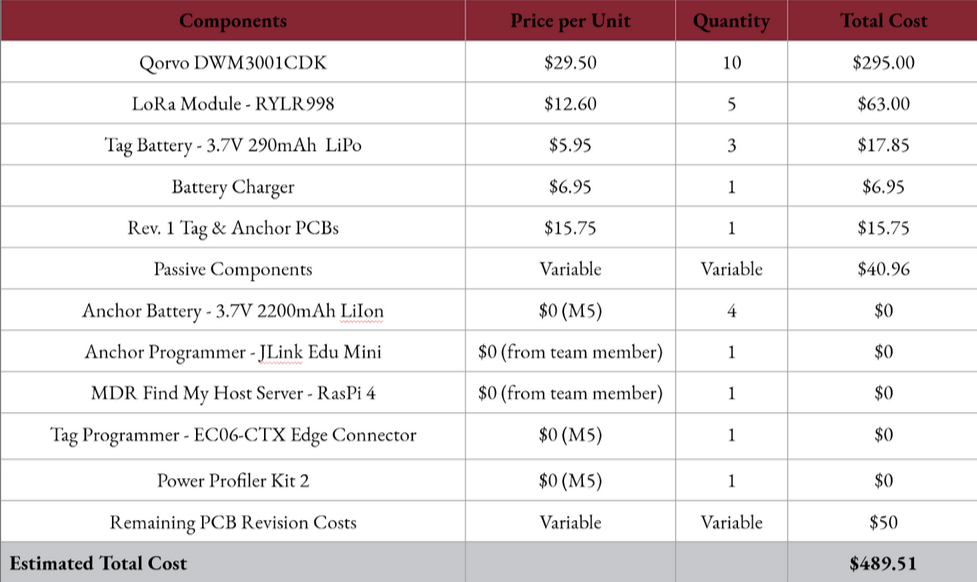
\includegraphics[scale=0.35]{mdr_project_expenditures.png}
\end{center}

\subsection{Project Management}
Team communication is done through text and Discord. We meet on a weekly 
basis both with each other and Professor Gummeson. GitHub and Google Drive 
are used as our version control platforms. Each team member has a unique 
skill-set that makes up for what another lacks, making the team dynamic 
optimal for a complex project. The experience of our team is evenly balanced 
with backgrounds in hardware and software, which is reflected in the 
designated project roles. 

\begin{itemize}
    \item Sean Brown - Logistics Lead and Hardware Support
    \item Connor McGarry - Hardware Lead
    \item Ken Su - Budget Lead and Software Support
    \item Walter Tebbetts - Software Lead
\end{itemize}

Varying levels of class workload makes it difficult for progress reports 
occasionally, but we try to log our progress for team review as best as 
possible. Each team member exercises leadership skills when another is too 
busy with external responsibilities to work on their designated part of the 
project for a while. Each team member understanding every aspect of the 
project has been important in helping each other out and making up for 
occasional slow progress. The largest hurdle we have overcome thus far is 
that of individual motivation and understanding of a team project. Some of 
us had not worked on a project of this scale before and therefore have 
needed to learn how to make careful decisions that affect other team members. 
Taking accountability in a team is another skill we are learning, as there 
have been a number of errors made where the best solution was to admit to 
the issue as soon as possible, and then collaborate on how to solve it. 

\subsection{Beyond the Classroom}
Classes that have been essential to this project so far have been ECE523, 
ECE325, ECE304 and ECE545. These classes relate to embedded system power 
management and networking, both of which are integral to the design of our 
project. We plan on having discussions with the professors of these classes 
as we progress in our development.

We have had to do more detailed data sheet analysis than what we did in 
ECE304, and Digikey has been an essential resource for component sourcing 
and information retrieval. 

We have used a variety of unfamiliar software and hardware in the project, 
all of which have required detailed research and experimentation. Since we 
have taken inspiration from GtHub projects, we have also spent a lot of time 
analyzing unfamiliar code to make sure we understand what we are using, and 
ensuring we are able to edit it according to our desired optimizations. 




\end{document}
